\documentclass[12pt, letterpaper]{../assignment}
\usepackage{graphicx}
\usepackage{courier}
\usepackage{minted}
\usepackage{amsmath}
\usepackage{commath}
\usepackage{amssymb}
\usepackage{amsfonts} 
\usepackage{cancel}
\usepackage{enumitem}
\usepackage{array}

\usepackage{tikz}
\usetikzlibrary{shapes,arrows,positioning}

\usemintedstyle{monokai}
\oddsidemargin = 0pt
\exercisesheet{Module 7}{Practice Assignment}
\student{Austin Barrilleaux}
\courselabel{EN 525.609}
\semester{Fall 2023}
\usepackage[backend=bibtex,style=numeric,sorting=none]{biblatex}
\bibliography{reference}
\usepackage{color}
\definecolor{light-gray}{rgb}{0.2,0.2,0.2}
\setminted{bgcolor=light-gray}
\setlength{\parindent}{0pt}

\makeatletter
\patchcmd{\minted@colorbg}{\noindent}{\medskip\noindent}{}{}
\apptocmd{\endminted@colorbg}{\par\medskip}{}{}
\makeatother

\begin{document}
\subsection*{Problem 1}
\subsubsection*{Solve the following practice problems in the 9th edition textbook.\\
\begin{itemize}
    \item Chapter 5:
    \begin{itemize}
        \item 5-3 (b,d,f)
        \item 5-4 (c,d)
    \end{itemize}
\end{itemize}}

\subsubsection*{5-3. Determine the step, ramp,
and parabolic error constants of the following unity-feedback control systems.
The forward-path transfer functions are given.}

\subsubsection*{(b) \ \  $ \mathbf{ G(s) = \dfrac{100}{s (s^2 + 10 s + 100)}}$}

The step error constant $K_p$, is calculated as:

$$ K_p = \lim_{s \to 0} \left[ G(s) \right]
       = \lim_{s \to 0} \left[ \frac{100}{s (s^2 + 10 s + 100)} \right]
       = \frac{100}{0}
       = \infty $$

The ramp error constant $K_v$, is calculated as:

$$ K_v = \lim_{s \to 0} \left[ s G(s) \right]
        = \lim_{s \to 0} \left[ \cancel{s} \frac{100}{\cancel{s} (s^2 + 10 s + 100)} \right]
        = \frac{100}{100}
        = 1 $$

The parabolic error constant $K_a$, is calculated as:

$$ K_a = \lim_{s \to 0} \left[ s^2 G(s) \right]
        = \lim_{s \to 0} \left[ \cancel{s} \cdot s \frac{100}{\cancel{s} (s^2 + 10 s + 100)} \right]
        = 0\left(\frac{100}{100}\right)
        = 0 $$

Therefore:

\begin{answer}
    $$ K_p = \infty, \ \ K_v = 1, \ \ K_a = 0  $$
\end{answer}

\subsubsection*{(d) \ \  $ \mathbf{ G(s) = \dfrac{100}{s^2 (s^2 + 10 s + 100)}}$}

The step error constant $K_p$, is calculated as:

$$ K_p = \lim_{s \to 0} \left[ G(s) \right]
       = \lim_{s \to 0} \left[ \frac{100}{s^2 (s^2 + 10 s + 100)} \right]
       = \frac{100}{0}
       = \infty $$

The ramp error constant $K_v$, is calculated as:

$$ K_v = \lim_{s \to 0} \left[ s G(s) \right]
        = \lim_{s \to 0} \left[ \cancel{s} \frac{100}{\cancel{s} \cdot s (s^2 + 10 s + 100)} \right]
        = \frac{100}{0}
        = \infty $$

The parabolic error constant $K_a$, is calculated as:

$$ K_a = \lim_{s \to 0} \left[ s^2 G(s) \right]
        = \lim_{s \to 0} \left[ \cancel{s^2} \frac{100}{\cancel{s^2} (s^2 + 10 s + 100)} \right]
        = \frac{100}{100}
        = 1 $$

Therefore:

\begin{answer}
    $$ K_p = \infty, \ \ K_v = \infty, \ \ K_a = 1  $$
\end{answer}

\subsubsection*{(d) \ \  $ \mathbf{ G(s) = \dfrac{K(1 + 2s)(1 +4s)}{s^2(s^2 + s + 1)}}$}

The step error constant $K_p$, is calculated as:

$$ K_p = \lim_{s \to 0} \left[ G(s) \right]
       = \lim_{s \to 0} \left[ \frac{K(1 + 2s)(1 +4s)}{s^2(s^2 + s + 1)} \right]
       = \frac{K (1) (1)}{0}
       = \infty $$

The ramp error constant $K_v$, is calculated as:

$$ K_v = \lim_{s \to 0} \left[ s G(s) \right]
        = \lim_{s \to 0} \left[ \cancel{s} \frac{K(1 + 2s)(1 +4s)}{\cancel{s} \cdot s (s^2 + s + 1)} \right]
        = \frac{K(1)(1)}{0}
        = \infty $$

The parabolic error constant $K_a$, is calculated as:

$$ K_a = \lim_{s \to 0} \left[ s^2 G(s) \right]
        = \lim_{s \to 0} \left[ \cancel{s^2} \frac{K(1 + 2s)(1 +4s)}{\cancel{s^2}(s^2 + s + 1)} \right]
        = \frac{K(1)(1)}{1}
        = K $$

Therefore:

\begin{answer}
    $$ K_p = \infty, \ \ K_v = \infty, \ \ K_a = K $$
\end{answer}

\subsubsection*{5-4. For the unity-feedback control systems described in Problem 5-2,
determine the steady-state error for a unit-step input,
a unit-ramp input, and a parabolic input, $\bold{(t^2/2)u_s(t)}$.
Check the stability of the system before applying the final-value theorem.}

\subsubsection*{(c) \ \  $ \mathbf{ G(s) = \dfrac{10(s + 1)}{s(s + 5)(s + 6)}}$}

The unity feedback transfer function is:

$$ M(s) = \frac{G(s)}{1+G(s)} = \frac{10\,s+10}{s^3+11\,s^2+40\,s+10} $$

Using the \texttt{roots()} function in MATLAB, we can see that the poles are:

$$ \texttt{roots([1,11,40,10])} = \left[ \begin{array}{cc} 
    -5.3653 &+ 2.8848i\\
    -5.3653 &- 2.8848i\\
    -0.2695 &+ 0.0000i
\end{array} \right] $$

\begin{answer}
All poles are in the left-hand plane (LHP). Therefore, the system is \textbf{stable}.
\end{answer}

The step error constant $K_p$, is calculated as:

$$ K_p = \lim_{s \to 0} \left[ G(s) \right]
       = \lim_{s \to 0} \left[ \frac{10(s + 1)}{s(s + 5)(s + 6)} \right]
       = \frac{10}{0}
       = \infty $$

The steady state error for a unit-step input, ${e_{\text{ss}_\text{p}}}$, is calculated as:

\begin{answer}
$$ {e_{\text{ss}_\text{p}}} = \frac{1}{1 + K_p} = \frac{1}{1 + \infty} = 0 $$
\end{answer}

The ramp error constant $K_v$, is calculated as:

$$ K_v = \lim_{s \to 0} \left[ s G(s) \right]
       = \lim_{s \to 0} \left[ \frac{10\cancel{s}(s + 1)}{\cancel{s}(s + 5)(s + 6)} \right]
       = \frac{10}{30}
       = \frac{1}{3} $$

The steady state error for a unit-ramp input, ${e_{\text{ss}_\text{v}}}$, is calculated as:

\begin{answer}
$$ {e_{\text{ss}_\text{v}}} = \frac{1}{K_v} = \frac{1}{1/3} = 3 $$
\end{answer}

The parabolic error constant $K_a$, is calculated as:

$$ K_a = \lim_{s \to 0} \left[ s^2 G(s) \right]
       = \lim_{s \to 0} \left[ \frac{10\cancel{s}s(s + 1)}{\cancel{s}(s + 5)(s + 6)} \right]
       = \frac{0}{30}
       = 0 $$

The steady state error for a parabolic input, ${e_{\text{ss}_\text{a}}}$, is calculated as:

\begin{answer}
$$ {e_{\text{ss}_\text{a}}} = \frac{1}{K_a} = \frac{1}{0} = \infty $$
\end{answer}

Overall the unit-step, unit-ramp, and parabolic input steady state error for the system are:

\begin{answer}
    $$ {e_{\text{ss}_\text{p}}} = 0, \ \ {e_{\text{ss}_\text{v}}} = 3, \ \ {e_{\text{ss}_\text{a}}} = \infty $$
\end{answer}

\subsubsection*{(c) \ \  $ \mathbf{ G(s) = \dfrac{100(s - 1)}{s^2(s + 5)(s + 6)^2}}$}

The unity feedback transfer function is:

$$ M(s) = \frac{100\,s-100}{s^5+17\,s^4+96\,s^3+180\,s^2+100\,s-100} $$

Using the \texttt{roots()} function in MATLAB, we can see that the poles are:

$$ \texttt{roots([1,17,96,180,100,-100])} = \left[ \begin{array}{cc} 
    -7.1437 &+ 1.9796i\\
    -7.1437 &- 1.9796i\\
    -1.5948 &+ 1.1275i\\
    -1.5948 &- 1.1275i\\
     0.4771 &+ 0.0000i
\end{array} \right] $$

\begin{answer}
    There is a single pole in the right-hand plane (RHP).
    Therefore, the system is \textbf{unstable}, so \textbf{an error analysis would be meaningless}.
    There is no need to perform the analysis.
    \textbf{The steady state error is infinite.} 
\end{answer}

\subsection*{Problem 2}
\subsubsection*{Consider the block diagram of the following missile attitude control system:}

\begin{figure}[H]
    \centering
    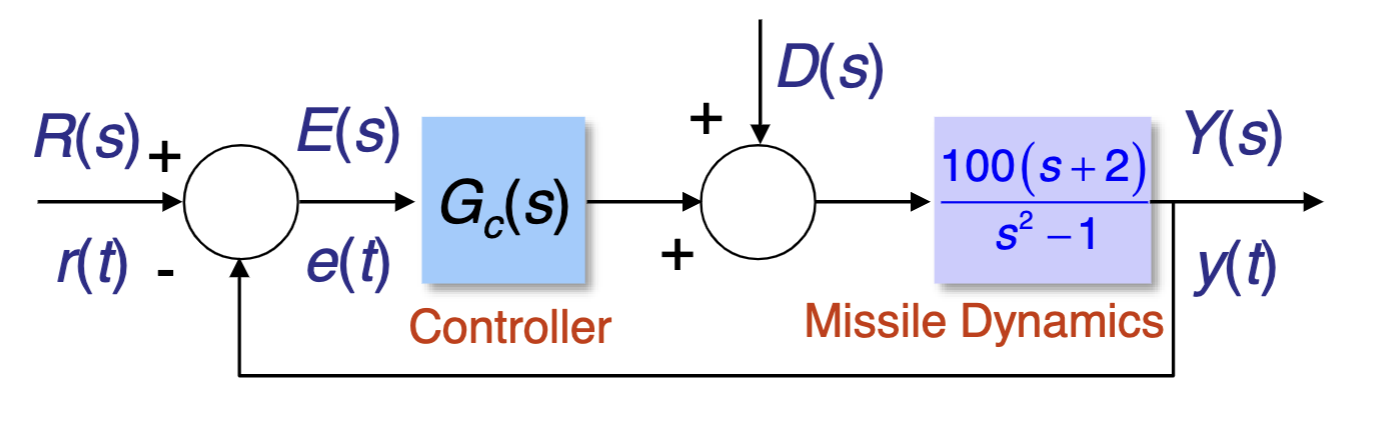
\includegraphics[width=0.7\linewidth]{./figures/Q2_diagram.png}
    \caption{Missile Attitude Control System}
    \label{fig:q2}
\end{figure}

\subsubsection*{(a) Let \boldmath{$G_c(s)=1$}, and find the SSE when \boldmath{$r(t)$} is a unit-step function.}

For this system:

$$ G(s) = \frac{100(s+2)}{(s^2 -1)} $$

The transfer function for the system is:

$$ \frac{Y(s)}{R(s)} = \frac{100\,s+200}{s^2+100\,s+199} $$

Using the \texttt{roots()} function in MATLAB, we can see that the poles are:

$$ \texttt{roots([1,17,96,180,100,-100])} = \left[ \begin{array}{cc} 
    -97.9687 &+ 0.0000i\\
    -2.0313 &+ 0.0000i
\end{array} \right] $$

All poles are in the left-hand plane (LHP). Therefore, the system is \textbf{stable}.

The step error constant $K_p$, is calculated as:

$$ K_p = \lim_{s \to 0} \left[ G(s) \right]
       = \lim_{s \to 0} \left[ \frac{100(s+2)}{(s^2 -1)} \right]
       = \frac{100(2)}{-1}
       = -200 $$

The steady state error for a unit-step input, ${e_{\text{ss}_\text{p}}}$, is calculated as:

\begin{answer}
$$ {e_{\text{ss}_\text{p}}} = \frac{1}{1 + K_p} = \frac{1}{1 + (-200)} = \frac{1}{-199} = -0.005 $$
\end{answer}

We can validate this by plotting the step response in MATLAB using the \texttt{step()} function,
which produces the following figure:

\begin{figure}[H]
    \centering
    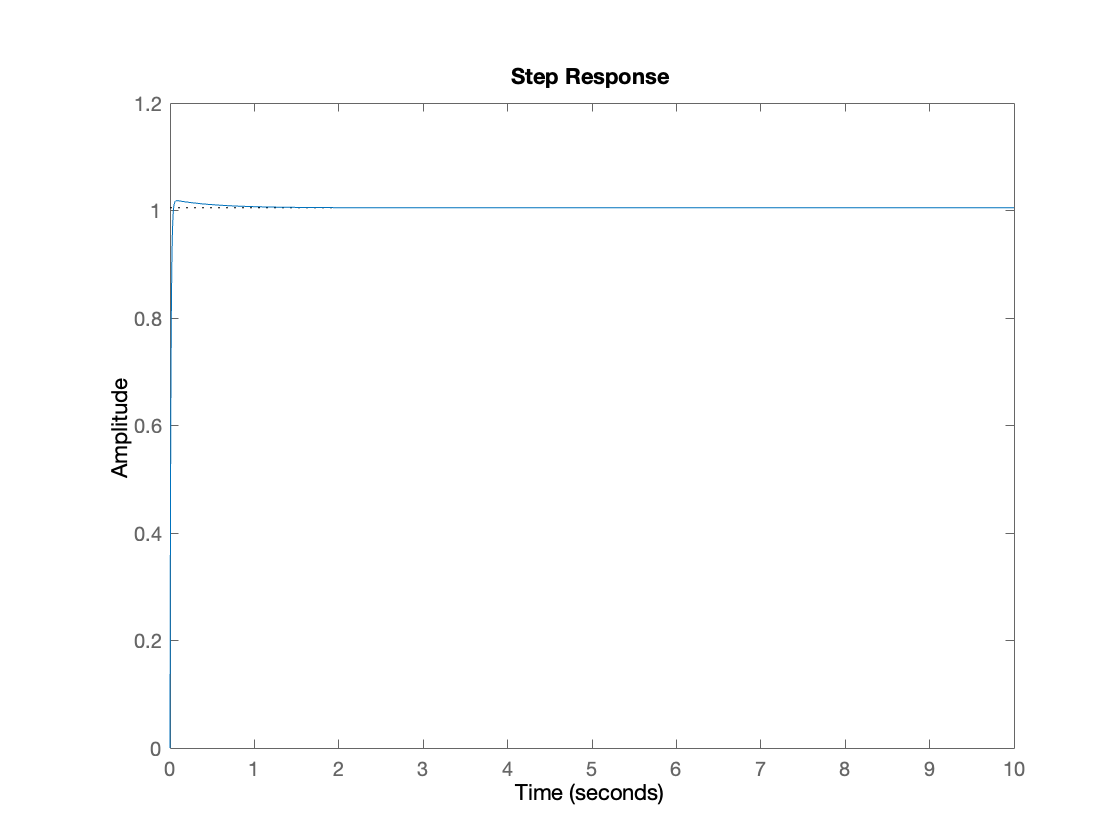
\includegraphics[width=0.7\linewidth]{./figures/Q2a_plot.png}
    \caption{$G_c (s) = 1$, Step Response}
    \label{fig:q2a_step}
\end{figure}

The last value of $y(t)$ at the end of the plot is $y(t=10) = 1.0050$, and the reference signal is 1.
Since:

$$ e(t) = \text{refernece signal} - y(t) $$

We can see that our above analysis resulted in the correct steady state error:

$$ e(t) = 1 - 1.0050 = -0.005 $$ 

\subsubsection*{(b) Let \boldmath{$G_c(s)=\frac{(s+\alpha)}{s}$}, and find the SSE when \boldmath{$r(t)$} is a unit-step function}

For this system:

$$ G(s) = \frac{100(s+2)(s+\alpha)}{s(s^2 -1)} $$

$$ \frac{Y(s)}{R(s)} = \frac{100s^2 + (200 + 100 \alpha)s + 200 \alpha}{s^3+100\,s^2+(199+100 \alpha) \,s+200\,\alpha } $$

The stability of the system depends on the value of $\alpha$.

Evaluating the characteristic equation using Routh Hurwitz, we get the following table:

\begin{center}
    \begin{tabular}{ | m{2em} | m{15em}| m{15em} | } 
      \hline
      $\mathbf{s^3}$ & $1$ & $100 \alpha + 199$ \\ 
      \hline
      $\mathbf{s^2}$ & $100$ & $200 \alpha$ \\ 
      \hline
      $\mathbf{s^1}$ & $98 \alpha + 199$ & 0 \\ 
      \hline
      $\mathbf{s^0}$ & $200 \alpha$ & 0 \\ 
      \hline
    \end{tabular}
\end{center}

In order for there to be no sign changes in the left most column, for a stable system, $\alpha \geq 0$.
\\\\
When $\alpha \geq 0$, the step error constant $K_p$, is calculated as:

$$ K_p = \lim_{s \to 0} \left[ G(s) \right]
       = \lim_{s \to 0} \left[ \frac{100(s+2)(s+\alpha)}{s(s^2 -1)} \right]
       = \left\{\begin{array}{cl} -200 & \text{\ if\ \ }\alpha =0\\ \frac{200 \alpha}{0} = \infty & \text{\ if\ \ }\alpha > 0 \end{array}\right.$$

The steady state error for a unit-step input, ${e_{\text{ss}_\text{p}}}$, is calculated as:

\begin{answer}
$$ {e_{\text{ss}_\text{p}}}[\alpha = 0] = \frac{1}{1 + K_p} = \frac{1}{1 + (-200)} = \frac{1}{-199} = -0.005 $$
\end{answer}

\begin{answer}
$$ {e_{\text{ss}_\text{p}}}[\alpha > 0] = \frac{1}{1 + K_p} = \frac{1}{1 + \infty} = 0 $$
\end{answer}

\subsection*{Problem 3}
\subsubsection*{Consider the following non-unity feedback system:}

\begin{figure}[H]
    \centering
    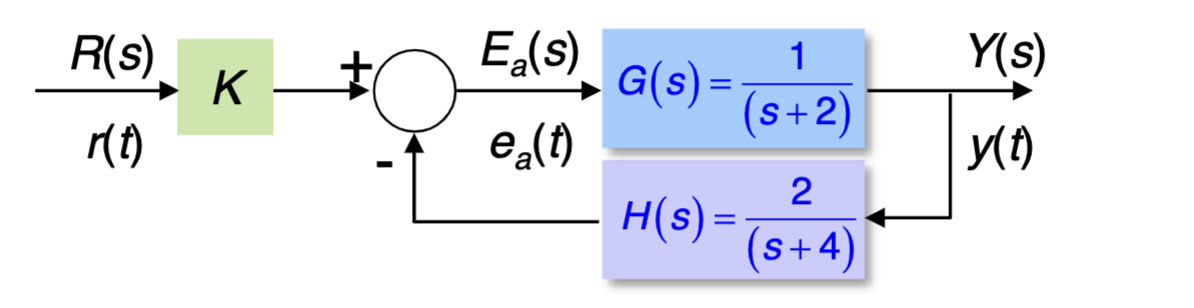
\includegraphics[width=0.7\linewidth]{./figures/Q3_diagram.png}
    \caption{Non-Unity System}
    \label{fig:q3}
\end{figure}

\subsubsection*{(a) Derive an equivalent unity-feedback forward path transfer function}


% \color{white}
% \hspace*{6em}\inputminted[frame=leftline,fontsize=\footnotesize]{matlab}
% {./matlab/Problem_5_18.m}
% \color{black}

% \begin{figure}[H]
%     \centering
%     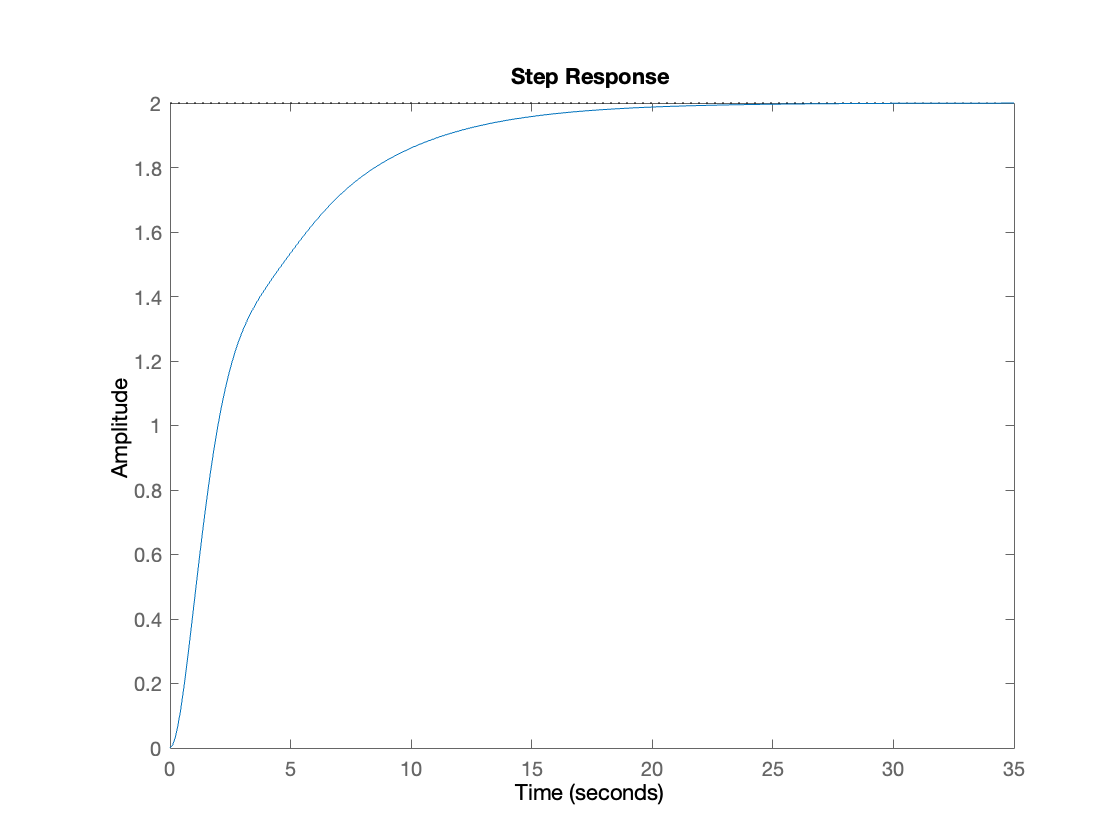
\includegraphics[width=0.7\linewidth]{./figures/step_response.png}
%     \caption{Step Response}
%     \label{fig:step}
%  \end{figure}



\end{document}

